\documentclass[a4paper,12pt]{article}

\usepackage{rotating}
\usepackage[top=1in, bottom=1in, left=0.75in, right=0.75in]{geometry}
\usepackage{graphicx}
\usepackage[numbers,square,sort&compress]{natbib}
\usepackage{setspace}
\usepackage[cdot,mediumqspace,]{SIunits}
\usepackage{caption}
\usepackage{subcaption}
\usepackage{mathtools}
\usepackage{authblk}
\usepackage{float}
\renewcommand{\thesubsection}{\thesection.\alph{subsection}}
\providecommand{\e}[1]{\ensuremath{\times 10^{#1}}}

\begin{document}
\onehalfspacing
\title{PHY 407 Lab 3}
\author{Natalie Price-Jones, 999091021}
\date{3 October 2014}
\affil{\small{natalie.price.jones@mail.utoronto.ca}}
\maketitle

\section{Question 1}

\subsection{Part b)}

The solution to

\[
\left[ \begin{array}{cccc}
0 & 1 & 4 & 1\\
3 & 4 & -1 & -1\\
1 & -4 & 1 & 5\\
2 & -2 & 1 & 3
\end{array} \right]
\mathbf{x} = 
\left[ \begin{array}{c}
-4 \\ 3 \\ 9 \\ 7
\end{array}\right],
\]

is given by 

\[
\mathbf{x} = \left[ \begin{array}{c}
 1.61904762 \\ -0.42857143 \\ -1.23809524 \\ 1.38095238
\end{array}\right]
\]

\section{Question 2}

\subsection{Part c)}

The Hamiltonian has the following energy eigenvalues for the first ten eigenstates: $E_0 = 5.83605893 eV$, $E_1 = 11.1801874 eV$, $E_2 = 18.66084476 eV$, $E_3 = 29.14053797 eV$, $E_4 = 42.64934576 eV$, $E_5 = 59.17700213 eV$, $E_6 = 78.71811979 eV$, $E_7 = 101.27080035 eV$, $E_8 =   126.83280052 eV$, $E_9 = 155.53240248 eV$.

\subsection{Part d)}

\begin{table}[H]
  \centering
  \begin{tabular}{|c||c||c||c|}
  \hline
  Energy State & H is $10 \times 10$ & H is $100 \times 100$ & Residual\\
  \hline
  \hline
   $E_0$ & 5.83605892708 & 5.83605852627 & $4.00801756228\e{-7}$\\
	\hline
	 $E_1$ & 11.1801874046 & 11.1801860811 & $1.32348002246\e{-6}$\\
	\hline
	 $E_2$ & 18.6608447561 & 18.6608428848 & $1.87132323148\e{-6}$\\
	\hline
	 $E_3$ & 29.1405379677 & 29.1405291667 & $8.8010350936\e{-6}$\\
	\hline
	 $E_4$ & 42.6493457585 & 42.6493366369 & $9.12161883093\e{-6}$\\
	\hline
	 $E_5$ & 59.1770021258 & 59.1769495345 & $5.25913648133\e{-5}$\\
	\hline
	 $E_6$ & 78.7181197916 & 78.7180679555 & $5.18361046034\e{-5}$\\
	\hline
	 $E_7$ & 101.270800354 & 101.27016932 & 0.000631034660444\\
	\hline
	 $E_8$ & 126.832800525 & 126.831967988 & 0.000832536703854\\
	\hline
	 $E_9$ & 155.532402483 & 155.402760328 & 0.129642155138\\
	\hline
  \end{tabular}
\label{tab:energy}
\end{table}

\begin{figure}[H]
\centering
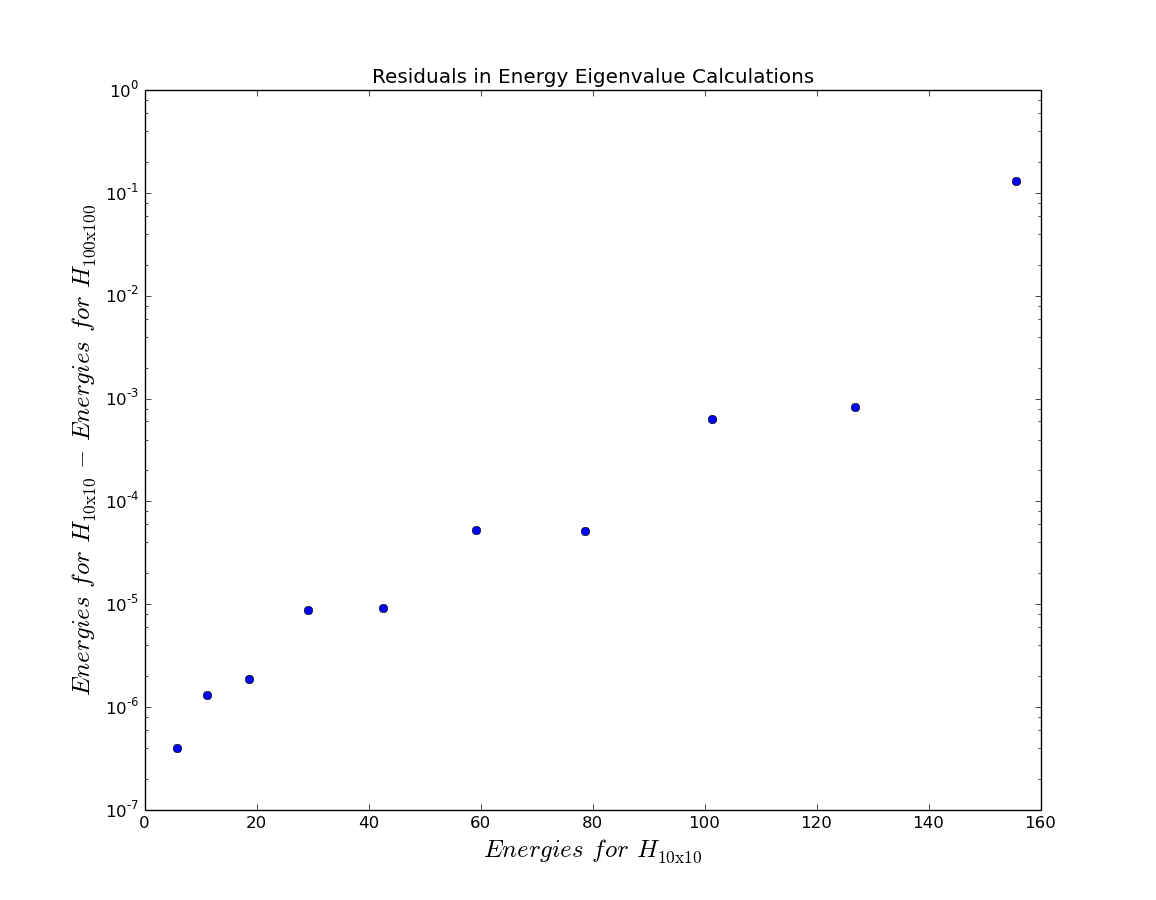
\includegraphics[width = \linewidth]{lab4q2d.png}
\caption{}
\label{fig:q2d}
\end{figure}

\subsection{Part e)}

BROKEN

\begin{figure}[H]
\centering
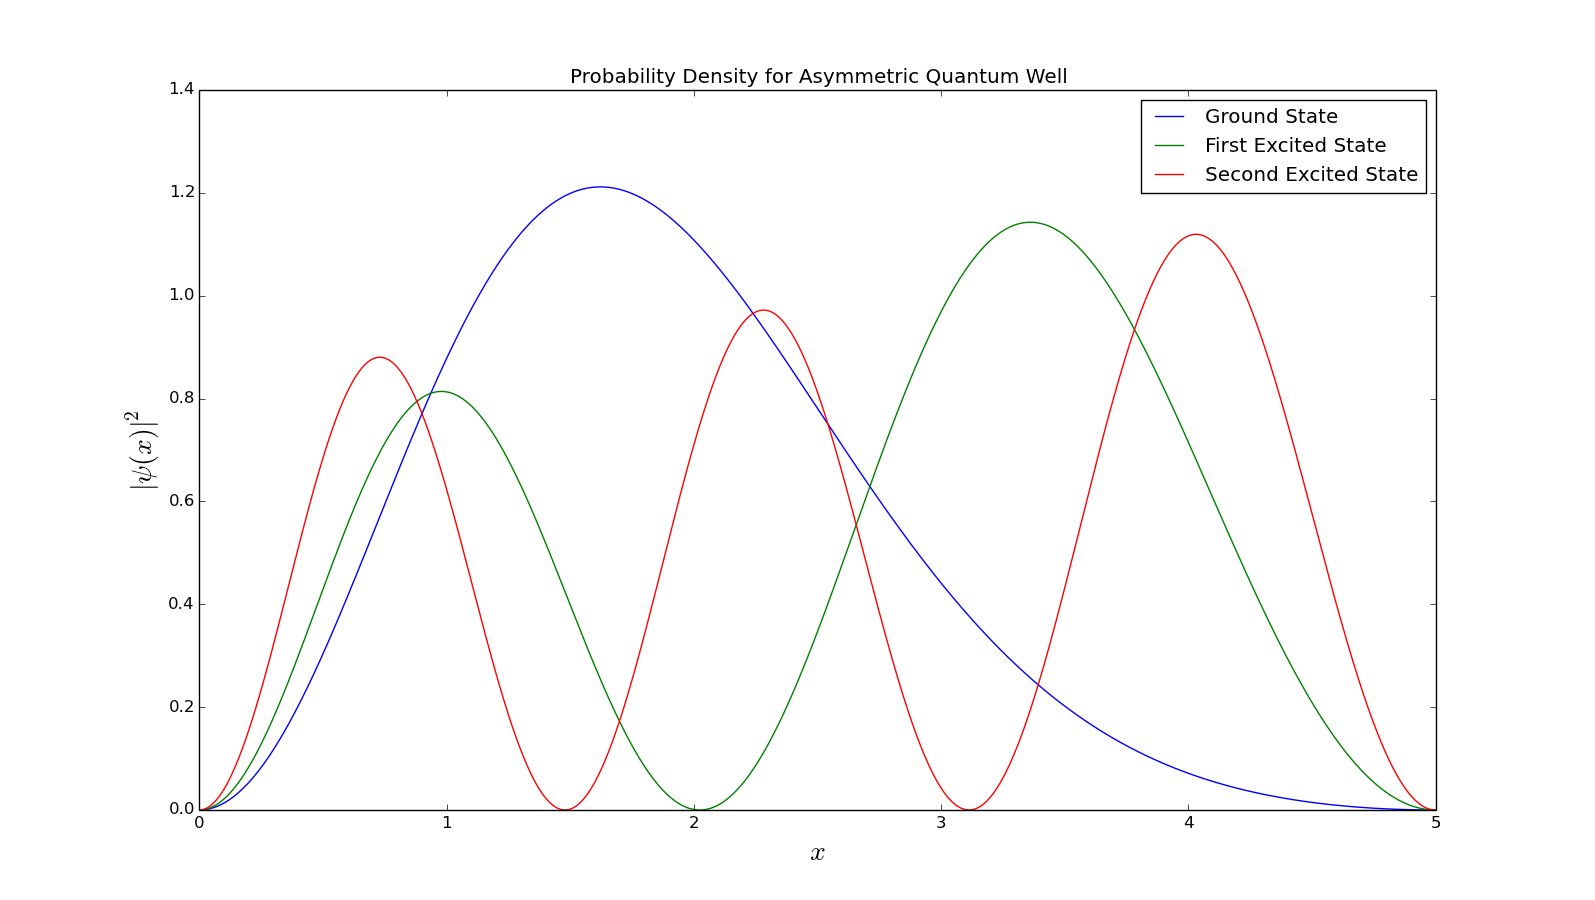
\includegraphics[width = \linewidth]{lab4q2ei.png}
\caption{}
\label{fig:q2ei}
\end{figure}

\begin{figure}[H]
\centering
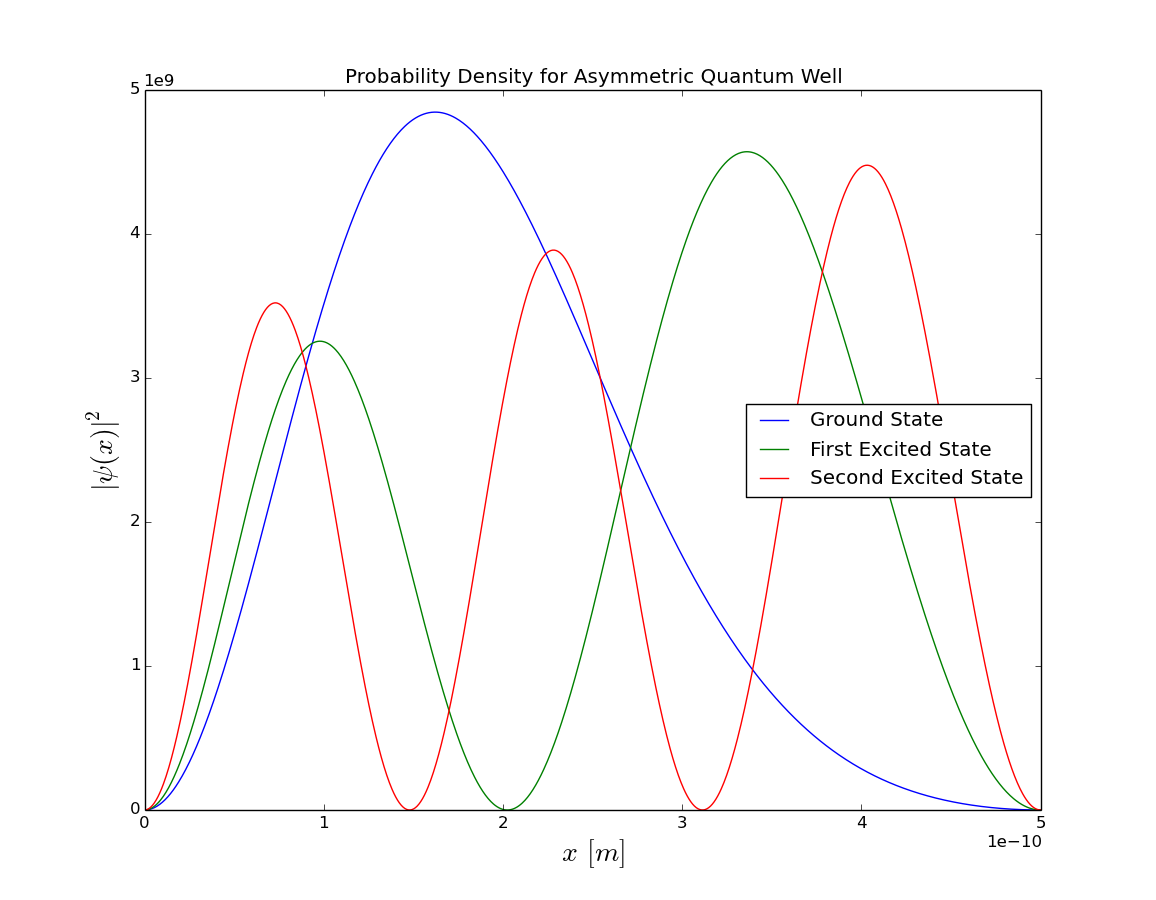
\includegraphics[width = \linewidth]{lab4q2ef.png}
\caption{}
\label{fig:q2ei}
\end{figure}

\section{Question 3}

\subsection{Part a)}

The solution to $x = 1 - e^{-cx}$ when $c = 2$ is $x = 0.796813$.

\subsection{Part b)}

\begin{figure}[H]
\centering
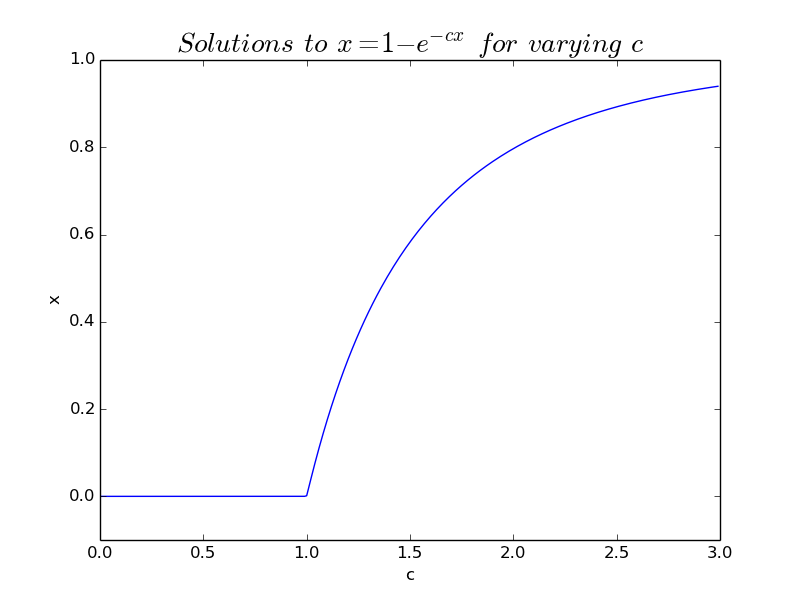
\includegraphics[width = \linewidth]{lab4q3b.png}
\caption{}
\label{fig:q3}
\end{figure}

\section{Question 4}

\subsection{Part a)}

We can show that the error in the overrelaxation method ($\epsilon '$), subject to some approximations, is given by:

\begin{eqnarray}
\epsilon'\simeq \frac{x-x'}{1 - 1/[(1+\omega)f'(x)-\omega]},\label{eqn:eps}
\end{eqnarray}

where $x'$ is the current solution, $x$ is the previous solution, $f(x)$ is the function equal to $x$ we are attempting to solve and $\omega$ is the parameter of the over relaxation.

We start with the definition of $x'$ for the over relaxation and the algebra follows from there.

\begin{eqnarray}
x' &=& x + (1+\omega)\Delta x = (1+\omega)f(x) - \omega x\nonumber\\
x' &=& (1+\omega)(f(x^*) + (x-x^*)f'(x^*) + ...) - \omega x \mathrm{\:\:\:(Taylor\;expand\;f(x))}\nonumber\\
x' &\simeq & (1+\omega)(x^* + (x-x^*)f'(x^*)) - \omega x \mathrm{\:\:\:(Drop\; higher\;order\;terms\;and\;use\;}x^* = f(x^*)\mathrm{)}\nonumber\\
x' &\simeq & x^* + \omega \epsilon - (1+\omega)\epsilon f'(x^*) \mathrm{\:\:\:(Used\;} x^* = x + \epsilon\mathrm{\;to\; rewrite\;} x^*-x)\nonumber\\
-\epsilon' &\simeq& \epsilon (\omega - (1+\omega)f'(x))\mathrm{\:\:\:(Used\;} x^* = x' + \epsilon' \mathrm{\; as\; above\; and\;} f'(x^*)\simeq f'(x)\mathrm{\; near\;} x^*)\nonumber\\
\implies \epsilon &\simeq& \frac{\epsilon'}{(1+\omega)f'(x) - \omega}\nonumber
\end{eqnarray}

Now substitute the expression for $\epsilon$ into $x^* = x + \epsilon$.

\begin{eqnarray}
x^* &\simeq& x + \frac{\epsilon'}{(1+\omega)f'(x) - \omega}\nonumber\\
x' + \epsilon' &\simeq& x + \frac{\epsilon'}{(1+\omega)f'(x^*)-\omega} \mathrm{\:\:\:(Since\;} x^* = x + \epsilon = x' + \epsilon')\nonumber\\
\epsilon'\left(1 - \frac{1}{(1+\omega)f'(x) - \omega}\right) &\simeq& x - x'\nonumber\\
\epsilon' &\simeq& \frac{x-x'}{1-1/[(1+\omega)f'(x) - \omega]}\nonumber 
\end{eqnarray}

So under the assumptions that $f(x)$ is well approximated by the first two terms of its Taylor series and that $f'(x^*)\approx f(x)$ near $x^*$, we have shown that Equation \ref{eqn:eps} is a good approximation of the uncertainty in the value $x'$ with respect to the true value.x

\subsection{Part c)}

When using over relaxation with $\omega = 0.5$, the result converged to the required accuracy in 4 iterations. Without this over relaxation, getting the required accuracy required 13 iterations. Some alternate guesses were made for $\omega$, but $0.5$ provided the most improvement over the regular relaxation method.

\subsection{Part d)}

\section{Question 5}

The following equation is satisfied by the $r =$ the $L1$ Lagrange point:

\begin{eqnarray}
\frac{GM}{r^2} - \frac{Gm}{(R-r)^2} &=& \omega^2r\nonumber\\
\implies \frac{GM}{r^2} - \frac{Gm}{(R-r)^2} - \omega^2r &=& 0
\label{eqn:lag}
\end{eqnarray}

Where $G$ is the gravitational constant, $M$ is mass of the Earth, $m$ is the mass of the Moon, $R$ is the distance between the Earth and the Moon and $\omega$ is the angular velocity of the Moon about the Earth.

The calculated value of the $L1$ Lagrange point using the secant method is $3.260\e{8}$ m. Setting $r = L1$ means Equation \ref{eqn:lag} evaluates to $3.579\e{-6}$, which is certainly close to zero.

\section{Question 6}

The effeciency $\eta$ of an incandescent bulb at a particular temperature $T$ is given by:

\begin{eqnarray}
\eta = \frac{15}{\pi^4}\int_{hc/\lambda_2 k_B T}^{hc/\lambda_1 k_B T} \frac{x^3}{e^x - 1} dx,\nonumber
\end{eqnarray}

where $h$ is Planck's constant, $c$ is the speed of light in a vacuum, $k_B$ is the Boltzmann constant, $\lambda_1 = 390$ nm and $\lambda_2 = 750$ nm.

\subsection{Part a)}

\begin{figure}[H]
\centering
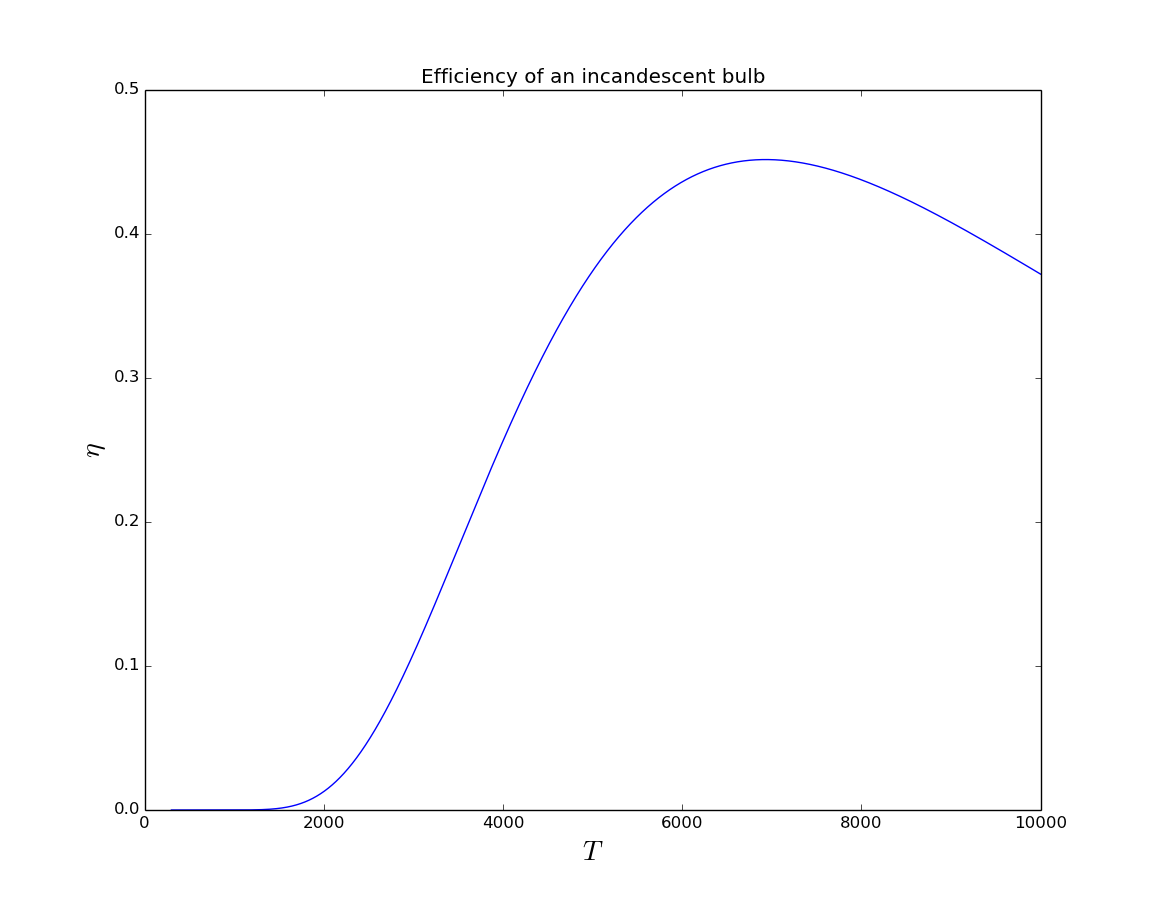
\includegraphics[width = \linewidth]{lab4q6a.png}
\caption{}
\label{fig:q6}
\end{figure}

\subsection{Part b)}

The maximum effieciency of Figure \ref{fig:q6} above occurs at $T = 6933.2087415$ K.

\end{document}





